\documentclass{article}

\usepackage{Sweave}
\begin{document}
\Sconcordance{concordance:Zischendetetkt2.tex:Zischendetetkt2.Rnw:%
1 2 1 1 0 1 1 1 2 1 0 9 1 1 6 5 0 1 1 3 0 1 2 1 4 1 2 1 1 1 3 1 2 3 1}

\begin{Schunk}
\begin{Sinput}
> library(jsonlite)
> library(ggplot2)
> library(dplyr)
> library(RColorBrewer)
> json_file<-'C:/LucMiaz/KG_dev_branch/KG/Measurements_example/MBBMZugExample/results/test_ZischenDetetkt2_2.0s_3000Hz_0dB_20-10-2015_14-59-39.json'
> dataraw<-fromJSON(json_file)
> tf<-dataraw$R
> tf <- filter(tf, !is.nan(BPR))
> tprfpr <- data.frame(TPR=double(), FPR=double(),threshold=double())
> authors=paste(unique(tf$author), sep=", ")
> for(i in seq(0.1,1,0.01)){
+   result<- tf$BPR<i
+   tf<-tf %>% mutate_(leqBPR=paste(as.numeric(result)))
+   len<-length(tf$leqBPR[!is.na(tf$leqBPR)])
+   tprfpr <- rbind(tprfpr,data.frame(TPR=sum(tf$leqBPR[tf$disc==1 & !is.na(tf$leqBPR)])/len, FPR=sum(tf$leqBPR[tf$disc==0 &!is.na(tf$leqBPR)])/len, threshold=i))
+ }
> tf$leqBPR<- NULL
\end{Sinput}
\end{Schunk}
\begin{figure}
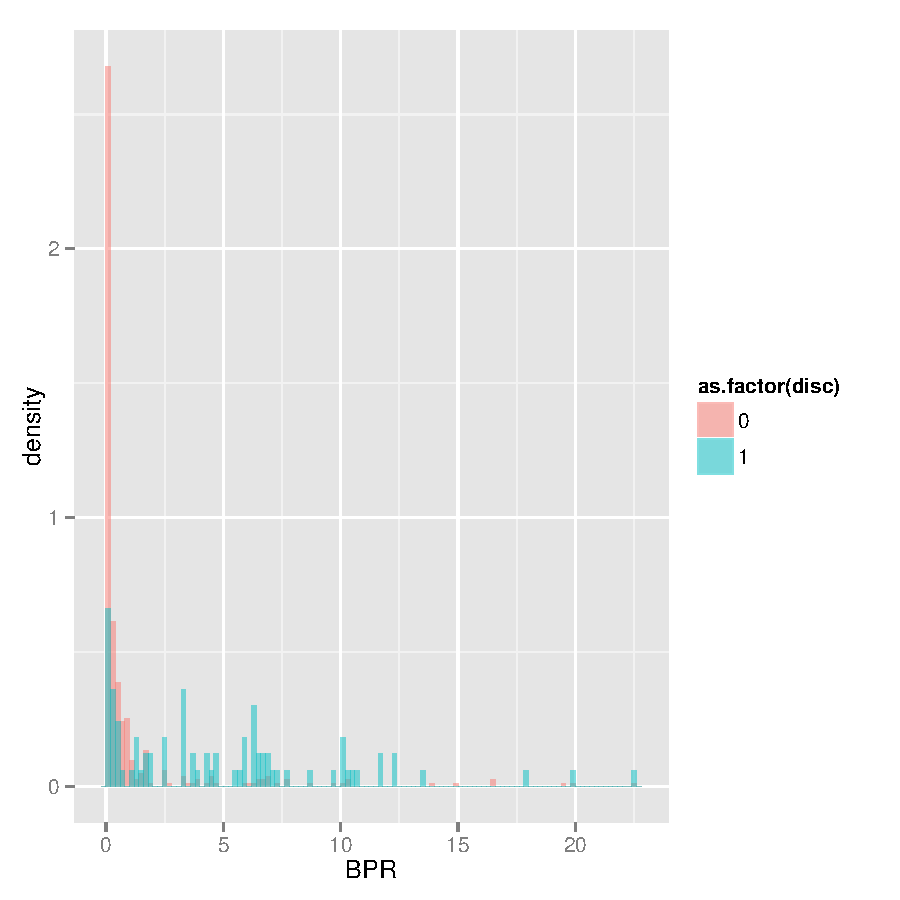
\includegraphics{Zischendetetkt2-002}
\end{figure}
\begin{figure}
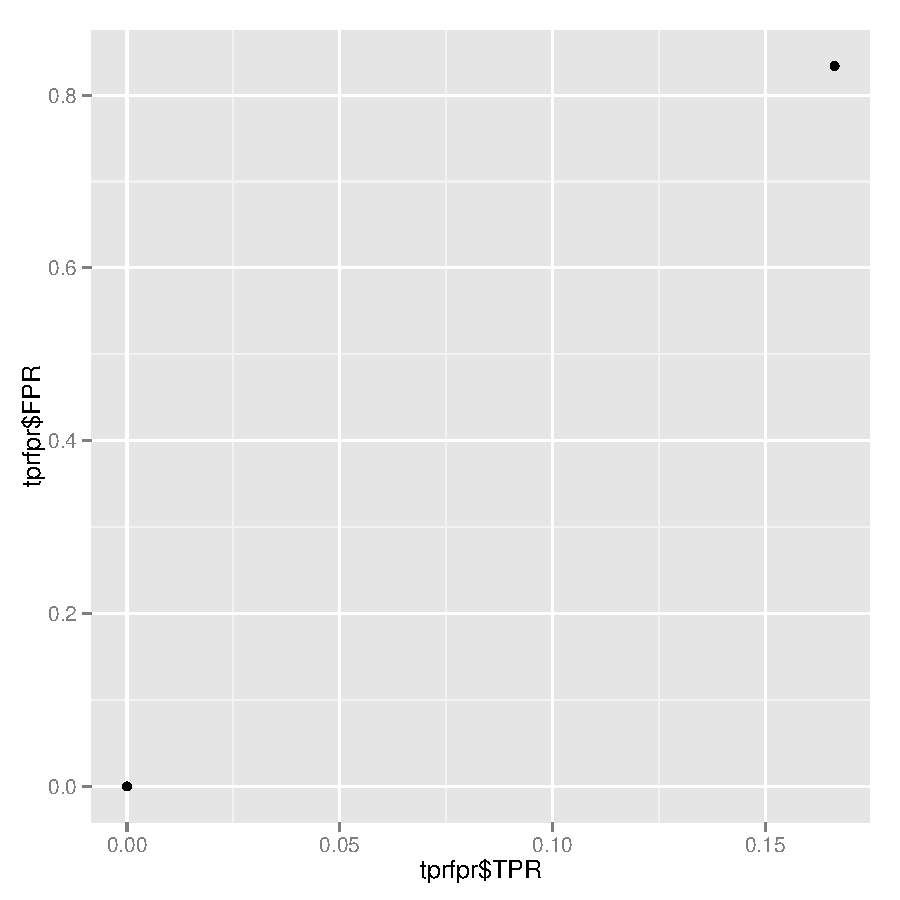
\includegraphics{Zischendetetkt2-003}
\end{figure}


\end{document}
